\documentclass[10pt]{beamer}
\usepackage[T1]{fontenc}
\usepackage{lmodern}
\usepackage[utf8]{inputenc}
\usepackage[spanish,es-tabla,es-noquoting,es-nodecimaldot]{babel}
\usepackage{amsmath,amssymb}
\usepackage{graphicx}
\usepackage{booktabs}

\usetheme{Madrid}
\usecolortheme{default}
\setbeamertemplate{navigation symbols}{}
\setbeamertemplate{footline}[frame number]

\graphicspath{{../notebooks/artifacts/}{./}}

\title[RL RoboCup 2D]{Persecución e Intercepción de Balón en RoboCup 2D con Q-Learning Tabular}
\subtitle{Fase 1 (P1) --- Grupo N\textdegree{} 1}
\author[Grupo 1]{Leonardo Candio \and Dimael Rivas}
\institute[UTEC]{DS5345 $\cdot$ Aprendizaje por Refuerzo (2026-II) \\ Docente: Percy W. Lovón Ramos}
\date{}

\begin{document}

\begin{frame}
    \titlepage
    \begin{center}
        \small Repositorio: \url{https://github.com/artrivas/RL-Project}
    \end{center}
\end{frame}

\begin{frame}{Tarea acotada: Ball Pursuit}
    \begin{itemize}
        \item El jugador parte de posición y orientación arbitrarias, con el balón inmóvil a $d_0 \in [5, 40]$\,m.
        \item Debe capturarlo ($d \le 0.8$\,m) en el menor tiempo posible.
        \item \textbf{Criterio de éxito:} tasa de captura $> 90$\,\% en menos de 40 pasos.
        \item Entorno principal: el cinemático del \textit{starter kit} del curso.
        \begin{itemize}
            \item \texttt{DASH 100} avanza 1.0\,m, \texttt{DASH 50} avanza 0.5\,m.
            \item \texttt{TURN $\pm$35} gira $\pm 35^\circ$ exactos, sin inercia ni ruido.
        \end{itemize}
        \item Dos distribuciones de inicio: $d_0$ uniforme en [5, 40]\,m y reset del kit ($d_0 \approx$ 11--19\,m).
    \end{itemize}
\end{frame}

\begin{frame}{MDP: estados y acciones}
    \textbf{Estados:} $s = (b_d(d),\, b_\theta(\theta))$ más terminal de captura.
    9 zonas de distancia $\times$ 11 sectores de rumbo = \textbf{99 estados}, 396 valores $Q$.
    \begin{itemize}
        \item Rumbo: bordes en $\pm 2.5^\circ$, $\pm 7.5^\circ$, $\pm 17.5^\circ$, $\pm 35^\circ$, $\pm 90^\circ$.
        Justificados por la tolerancia angular $\arcsin(0.8/d)$ y la mitad del giro ($17.5^\circ$).
        \item Distancia: bordes en 3, 6, 10, 15, 20, 25, 30, 35\,m (3--5 pasos por zona).
    \end{itemize}
    \textbf{Acciones:} \texttt{DASH 100}, \texttt{DASH 50}, \texttt{TURN +35}, \texttt{TURN $-$35}.
\end{frame}

\begin{frame}{MDP: transiciones, recompensa y descuento}
    \begin{itemize}
        \item \textbf{Transiciones:} deterministas en $(\mathbf{x}, \phi)$, estocásticas sobre los bins
        (aliasing: un mismo bin agrupa posiciones con distinto futuro).
        \item \textbf{Recompensa} (enunciado):
        $r_t = (d_t - d_{t+1}) - 0.2 + 100 \cdot \mathbb{1}\{d_{t+1} \le 0.8\}$.
        Con captura, maximizar $G_0$ equivale a capturar en menos pasos.
        \item \textbf{Descuento:} $\gamma = 0.99$ (el bono vale 67.6 en el paso 39; con 0.9 valdría 1.6).
        Truncamiento en 40 pasos con bootstrap desde $s'$.
    \end{itemize}
\end{frame}

\begin{frame}{Algoritmo e hiperparámetros}
    \textbf{Q-Learning:} $Q(s,a) \leftarrow Q(s,a) + \alpha[r + \gamma \max_{a'} Q(s',a') - Q(s,a)]$,
    $\varepsilon$-greedy con desempate al azar.
    \begin{itemize}
        \item Comparación justa, mismo nivel final: $\varepsilon = 0.1$ constante vs.\
        $\varepsilon_k = \max(0.1,\, 1.0 \cdot d^k)$, $d = 0.999952$.
        \item $\alpha = 0.1$, $\gamma = 0.99$, 80\,000 episodios y 5 semillas por condición.
        \item Evaluación greedy cada 4\,000 episodios sobre 500 inicios fijos en [5, 40]\,m.
        \item Q-Learning, SARSA y Monte Carlo empatan ($\approx 85$\,\%); se reporta Q-Learning.
    \end{itemize}
\end{frame}

\begin{frame}{Resultado principal: ablación}
    \begin{table}
        \centering\scriptsize
        \begin{tabular}{@{}lcc@{}}
            \toprule
            Exploración & Final $<40$ en [5, 40]\,m & Reset del kit \\
            \midrule
            $\varepsilon$ decreciente & \textbf{0.857 $\pm$ 0.003} & \textbf{1.000}, 19.1 pasos \\
            $\varepsilon = 0.1$ constante & 0.843 $\pm$ 0.013 & 1.000, 19.3 pasos \\
            \midrule
            \textit{Óptimo exacto (A*)} & \textit{0.879} & \textit{1.000}, \textit{18.6 pasos} \\
            \bottomrule
        \end{tabular}
    \end{table}
    \begin{itemize}
        \item El decreciente llega al 80\,\% en 12\,000--16\,000 episodios; el constante en 16\,000--32\,000.
        \item \textbf{Ninguna política supera el 87.9\,\% en [5, 40]\,m} (óptimo exacto): el 90\,\% no es
        alcanzable allí; la nuestra llega al 97.5\,\% del óptimo.
    \end{itemize}
\end{frame}

\begin{frame}{Evaluación greedy durante el entrenamiento}
    \begin{center}
        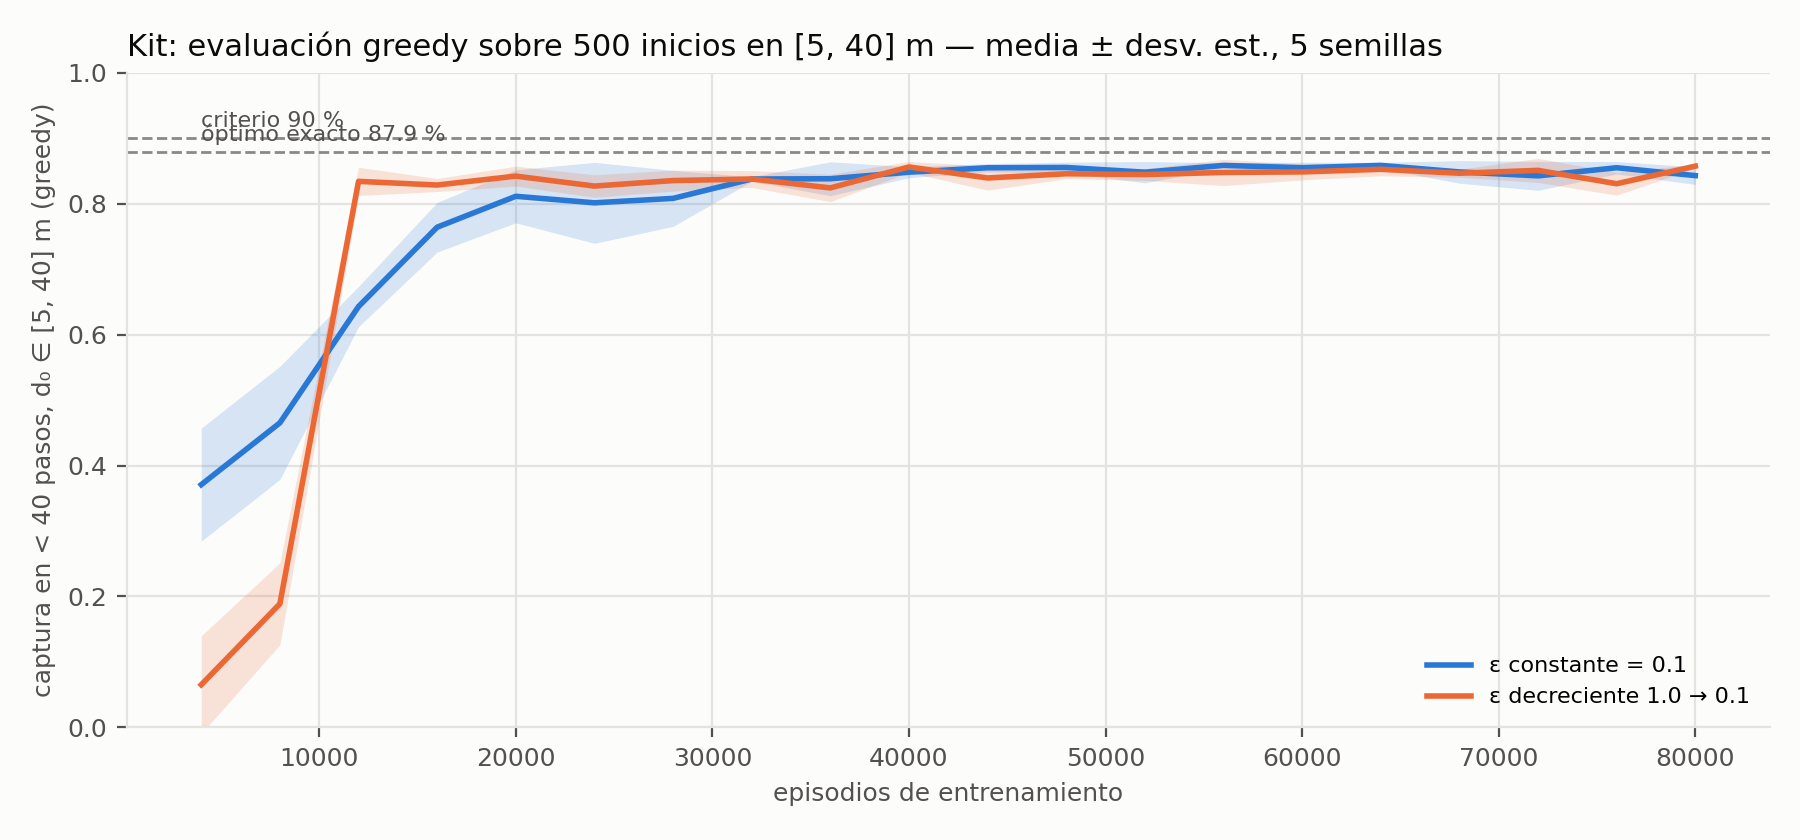
\includegraphics[width=0.85\textwidth]{fig_kit_eval.png}
    \end{center}
\end{frame}

\begin{frame}{Retorno y éxito en entrenamiento}
    \begin{center}
        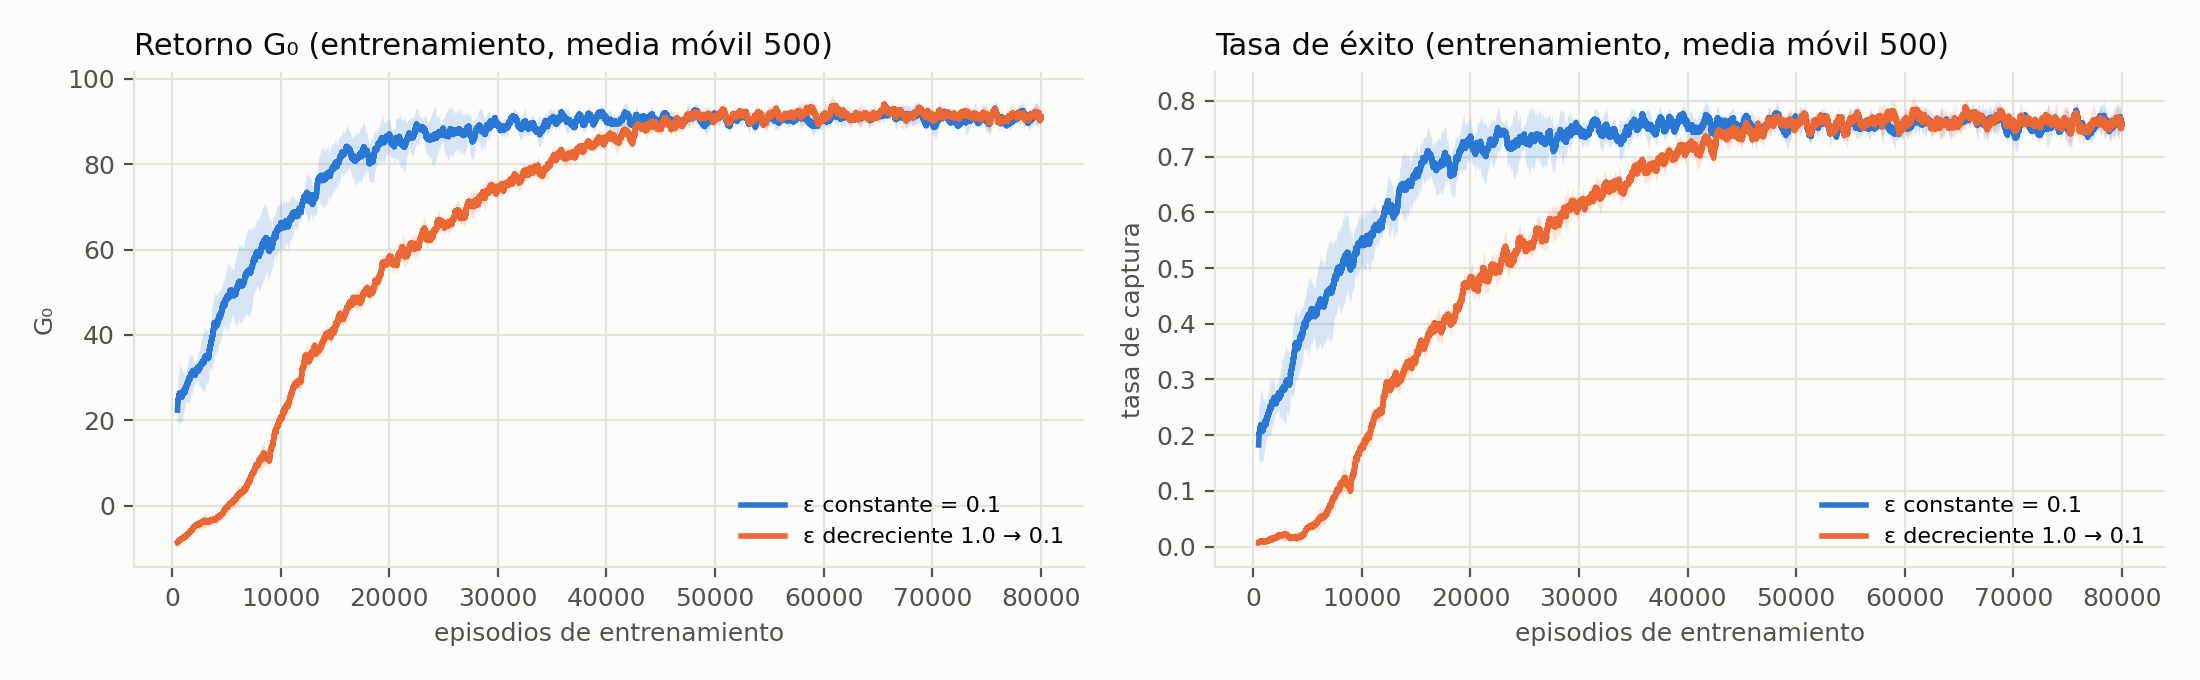
\includegraphics[width=\textwidth]{fig_kit_training.png}
    \end{center}
\end{frame}

\begin{frame}{Política y valor aprendidos}
    \begin{center}
        
\includegraphics[width=\textwidth]{fig_kit_policy_value.png}
    \end{center}
    \begin{itemize}
        \item Avanza con \texttt{DASH 100} entre $-35^\circ$ y $+17.5^\circ$; gira hacia el balón fuera de esa ventana.
    \end{itemize}
\end{frame}

\begin{frame}{Trayectorias: de erráticas a casi rectas}
    \begin{center}
        
\includegraphics[width=\textwidth]{fig_kit_learning_traj.png}
    \end{center}
\end{frame}

\begin{frame}{Transferencia a \texttt{rcssserver}}
    \begin{itemize}
        \item Política final ejecutada en el servidor real, 200 episodios por distribución, 0 comandos perdidos.
        \item Reset del kit: 26.0\,\% $\pm$ 3.1 en vivo (la física real difiere del kit: avance gradual,
        giro con velocidad, ruido, visión parcial).
        \item Política entrenada con física del servidor: \textbf{73.5\,\% $\pm$ 3.1} en vivo en [5, 40]\,m.
        \item Prueba de 500 episodios consecutivos sin errores de socket.
    \end{itemize}
\end{frame}

\begin{frame}{Otras tareas del catálogo (formulación)}
    \begin{table}
        \centering\scriptsize
        \begin{tabular}{@{}lccc@{}}
            \toprule
            & Conducción & Tiro & 2v1 \\
            \midrule
            $|\mathcal{S}|$ & 108 & 36 & 324 \\
            $|\mathcal{A}|$ & 4 & 6 & 4 \\
            $|\mathcal{S}|\times|\mathcal{A}|$ & 432 & 216 & 1\,296 \\
            Criterio & $>30$\,m, $>80$\,\% & $>75$\,\% / $>50$\,\% & $>50$ pasos, $\ge 3$ pases \\
            \bottomrule
        \end{tabular}
    \end{table}
    \begin{itemize}
        \item Misma cinemática simple del kit; propuesta formulada, pendiente de implementar.
    \end{itemize}
\end{frame}

\begin{frame}{Conclusiones}
    \begin{itemize}
        \item MDP tabular de 99 estados con discretización justificada por la geometría de captura.
        \item $\varepsilon$ decreciente aprende antes y es más estable que el constante.
        \item Reset del kit: \textbf{100\,\% en todas las semillas} (19.1 pasos, óptimo 18.6).
        \item En [5, 40]\,m el 90\,\% es inalcanzable (óptimo 87.9\,\%); llegamos a 85.7\,\%.
        \item Ejecución verificada en \texttt{rcssserver}.
        \item P2: DQN/PPO continuos, entrenar con física del servidor, recompensa consistente con el descuento.
    \end{itemize}
\end{frame}

\end{document}
